\documentclass[a4paper,10pt]{report}
\usepackage[utf8]{inputenc}
\usepackage{graphicx}
\usepackage{fullpage}
\usepackage{verbatim}
\usepackage[spanish]{babel}
\usepackage{wrapfig}
\usepackage{url}
\usepackage[font={scriptsize}]{caption}
\setcounter{secnumdepth}{3}
\setcounter{tocdepth}{3}
\selectlanguage{spanish}


\title{Implementación en GPU de un algoritmo eficiente de dinámica molecular con potenciales numéricos}
\author{Ignacio Eguinoa \\ 
\small Facultad de Informática, UNLP
\date{}
}


\addtolength{\topmargin}{-35pt}
\addtolength{\textwidth}{80pt}
\addtolength{\textheight}{100pt}
\addtolength{\oddsidemargin}{-40pt}


\begin{document}

\maketitle



\section*{Resumen} 




En este trabajo se presentan modificaciones al algoritmo de dinámica molecular sobre GPU, basadas en la optimización del cálculo del potencial de Lennard-Jones.
Siguiendo las especificaciones del método encontradas en la literatura se implementa un algoritmo eficiente de dinámica molecular sobre GPU que evoluciona exlusivamente de acuerdo a un modelo de potencial de Lennard-Jones. 
Usando este desarrollo como referencia, se introducen adaptaciones para el cálculo del potencial y las fuerzas derivadas de éste, haciendo uso de valores tabulados y teniendo en cuenta tanto las propiedades de la función potencial como las características del hardware sobre el cual se trabaja.

Además de las mejoras en performance, se tiene en cuenta otro aspecto importante: la precisión numérica con la que se opera. Dado que la utilización de valores tabulados implica un error en el potencial y su fuerza resultante, es necesario evaluar la implicancia que tendrá esto sobre la correctitud de la simulación.

Las implementaciones actuales del método sobre arquitecturas GPU proveen una gran mejora en la performance con respecto a las versiones iniciales implementadas sobre CPU, lo cual es producto de las propiedades intrínsecamente paralelas del algoritmo y el gran poder de computo que ofrece la arquitectura altamente paralelizada del hardware. 
Por su parte, las adaptaciones realizadas en este trabajo presentan una optimización extra manteniendo la calidad númerica de los resultados. 

Dado que el potencial de Lennard-Jones representa un aporte importante para modelar las interacciones en distintos campos de fuerzas, las mejoras obtenidas pueden ser incorporadas fácilmente a una gran cantidad de versiones existentes de este método de simulación. 

Por último, los resultados obtenidos alientan a evaluar este tipo de aproximaciones para optimizar cálculos con formas funcionales similares en algoritmos que hayan sido implementados sobre GPU. De esta forma, se intenta explotar todas las propiedades que ofrece la arquitectura.


\pagebreak




\tableofcontents

\pagebreak


\chapter{Introducción}


\section{Objetivos}



El principal objetivo de la tesis es obtener una implementacion del método de dinámica molecular basada en GPU, que siga un modelo de interaccion de 
Lennard-Jones(potencial de no-union), y que resuelva el calculo de las fuerzas utilizando valores tabulados en el sistema de memoria provisto por la arquitectura. 

La forma funcional que describe el potencial de Lennard-Jones permitiria obtener una buena aproximación del valor utilizando una tabla de resultados precalculados. 
Además, el sistema de memorias de la arquitectura, que ha evolucionado considerablemente desde su creación de esta, permite recuperar de forma eficiente el valor asociado en un esquema de tablas. 
De esta forma, se espera que la modificacion resulte en una mejora de la performance manteniendo la correctitud en los resultados de la simulación. 



\section{El método de dinámica molecular}

\subsection{Fundamentos}


Los sistemas químicos de interés como las proteínas suelen ser complejos de estudiar debido a su gran tamaño. 
La superficie de energía libre, que describe la energía del sistema y a partir de la cual se podrían derivar todas las propiedades termodinámicas y cinéticas de interés, es una función 3N dimensional (siendo N el número de partículas del sistema), lo que hace imposible derivar analíticamente las propiedades por el altísimo costo computacional asociado.

Otra forma de analizar estos sistemas es mediante una aproximación numérica, a través de simulaciones computacionales.  	
La simulación computacional de biomoléculas involucra la exploración de su superficie de energía libre, la cual, debido a la complejidad de estos sistemas, es altamente accidentada, contiene una gran cantidad de mínimos locales y de barreras de energéticas. 
De esta forma, si los parámetros de la simulación están correctamente definidos, el conjunto de conformaciones adoptadas durante la ejecución será representativo del ensamble real de conformaciones posibles del sistema, lo que nos permite estimar las propiedades de interés.

Los métodos de simulación molecular nos permiten, entonces, obtener una serie de configuraciones representativas del sistema, de modo que las propiedades termodinámicas extraídas del mismo se correspondan de manera precisa con los valores reales.
Una de las formas de obtener estas configuraciones es mediante el método de dinámica molecular(DM). Este método implica simular la progresion temporal "real" del sistema, obteniendo distintas conformaciones a medida que avanza el tiempo de simulación.

La técnica de simulación de dinámica molecular se basa en resolver las ecuaciones de movimiento de Newton para cada átomo del sistema; así, en cada "paso" de la simulación se calcula la energia potencial entre las particulas y de ésta se derivan las fuerzas que actúan sobre cada átomo. 
Las ecuaciones de Newton relacionan las fuerzas resultantes del potencial con la aceleracion que tendra cada particula y, por lo tanto, el cambio en la velocidad y en la posicion con el tiempo. 
Dado que el potencial es una función continua dependiente de la posición, los cambios en las velocidades y posiciones resultan de una integracion a lo largo de la trayectoria de la partícula.


\subsection{Esquema general del método}

En la práctica, la integración de las ecuaciones de Newton se calcula computacionalmente mediante el llamado Algoritmo de Verlet, el cual resuelve la integración en una ecuación discreta donde las posiciones estan separadas por intervalos de tiempo ("dt") . 
Usando las fuerzas resultantes, junto con las posiciones y velocidades de las partículas correspondientes a la iteración, el algoritmo de Verlet calcula las nuevas posiciones y velocidades en un intervalo de tiempo posterior. De este modo se genera una trayectoria, determinada por las posiciones de las particulas en cada paso de la simulación. 
Esta trayectoria describe como cambia la conformación espacial del sistema a lo largo del tiempo. 
La elección del "dt" es una situación de compromiso, ya que un valor muy chico, si bien representa la propagación del movimiento de forma mas precisa(mas cercana al valor real de la integración), requiere una mayor cantidad de cálculos para un mismo tiempo total de simulación. 



El esquema general del método se puede ver en la figura \ref{esquemaMD}.

% **********************************************************************
% ***************CAMBIAR LA FIGURA POR UNA SIMILAR EN ESPAÑOL **********
% **********************************************************************

\begin{figure}[!ht]
\begin{center}
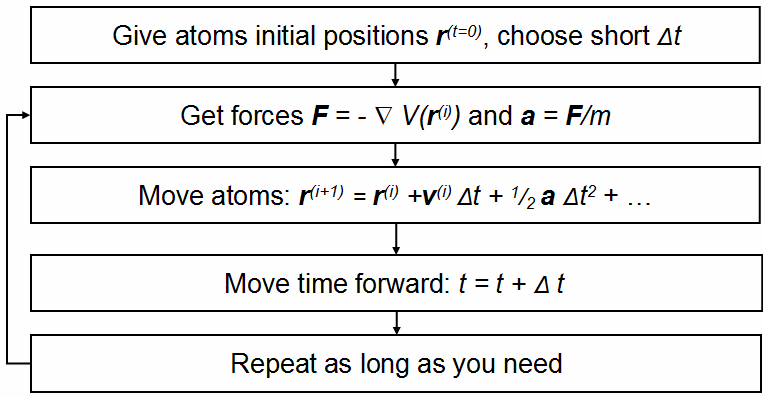
\includegraphics[keepaspectratio, width=0.5\textwidth]{img/mdalgorithm.png}
\end{center}
\caption{Esquema general del algoritmo de dinámica molecular}
\label{esquemaMD}
\end{figure}





% *********************
% ****QUE OTROS DATOS RELEVANTES OBTENGO DE LA SIMULACION??
%********************** 


El resultado de la simulación es, fundamentalmente, una trayectoria representada por las posiciónes de cada una de las partículas a lo largo de un cierto tiempo.
No se va a detallar acerca del procesamiento de este resultado pero es relevante decir que la longitud de trayectoria que podamos obtener en un tiempo de cómputo razonable es lo que limita el tipo de proceso químico que podremos estudiar.
Para poder estudiar un proceso de interés es necesario que la simulación alcance la escala de tiempo en la cual éste ocurre. Un mayor tiempo de simulación equivale a realizar más pasos y por lo tanto más cálculos totales, aumentando así el tiempo de cómputo requerido.

Por su parte, simular sistemas más grandes (con mayor cantidad de partículas) implica un incremento en la cantidad de cálculos por cada paso y por lo tanto un mayor costo computacional. Además, la función que describe las propiedades del sistema tiene por naturaleza una mayor cantidad de variables, debido a esto es necesario correr la simulación durante más tiempo para poder llegar a un conjunto de conformaciones que sea representativo del ensamble real.




\subsection{La función potencial}


En la utilización del método de dinámica molecular, el potencial(V) que permite derivar las fuerzas entre partículas se obtiene modelando al sistema molecular mediante la mecánica clásica (método conocido como mecánica molecular o MM).
Usando un método de MM, se ignoran los electrones y la naturaleza cuántica de estos. La energía potencial del sistema, entonces, depende exclusivamente de las posiciones de los núcleos atómicos. Se modela cada molécula como un conjunto de sitios -que representan los átomos que la componen- y resortes -que representan los enlaces químicos entre estos- junto con un potencial parametrizado ad hoc.
Este potencial es una función matemática que depende exclusivamente de las posiciones de los atomos, la cual se ajusta a las interacciones observadas experimentalmente entre los componentes del sistema. Este tipo de repesentacion simplificada del sistema permite reducir la complejidad de los cálculos necesarios para la simulación, y por lo tanto el costo computacional asociado, pero limita el tipo de procesos que se pueden estudiar. Por ej. no se pueden estudiar reacciones quimicas que impliquen ruptura o formación de enlaces ya que estos no son considerados con suficiente detalle.

Las interacciones representadas en el método de MM se pueden agrupar en dos tipos:

\begin{description}
 \item [De unión:] Describen las interacciones entre dos átomos unidos entre si directamente o hasta dos enlaces de distancia. 
 Consisten en aquellos términos del potencial cuya energía se ve afectada por los estiramientos de los enlaces, las flexiones de los ángulos entre dos átomos, y la rotación de dos átomos adyacentes sobre un eje (ángulos dihedros). Los estiramientos y las flexiones angulares son modeladas
mediante un oscilador armónico, mientras que las rotaciones de los enlaces en el plano son modeladas mediante una función trigonométrica.

\item [De no unión:] describen la interacción entre átomos ubicados a más de 3 enlaces de distancia de la misma molécula, o bien entre átomos de moléculas distintas, y consisten en un término para la
contribución electrostática calculada mediante la Ley de Coulomb, y un término para la contribución de Van Der Waals modelada por un potencial de Lennard-Jones 12-6.


\end{description}



El esquema general de la función potencial suele tomar una forma similar a la que sigue: \\
% 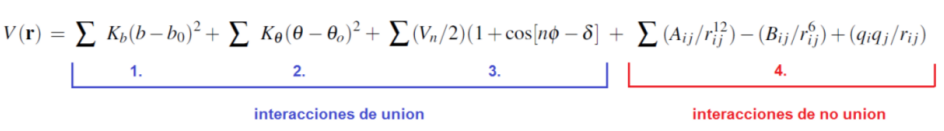
\includegraphics[]{img/ecPotencialAmber.png}
% \begin{figure}[h]
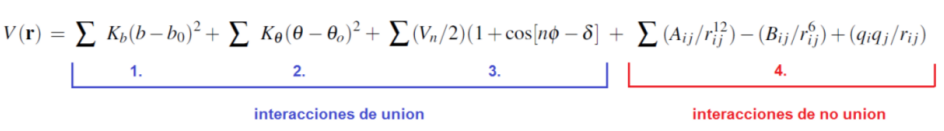
\includegraphics[keepaspectratio, width=1.0\textwidth]{img/ecPotencialAmber.png}
% \caption{Ejemplo de potencial de interacción del paquete de software Amber}
% \label{Fig:Amber}
% \end{figure}
\vspace{2pt}

En azul se representan los términos matemáticos que modelan las interacciones de unión (1. Término de estiramiento de enlaces; 2. Término de flexión angular; 3. Término de rotación de ángulos diedros), y en rojo
las interacciones de no unión (Potencial de Lennard-Jones 12-6 e interacción Coulómbica).

Los parámetros que se observan en esta función potencial (las constantes $K_b, K_{\theta}$ y $V_n$ , los valores de equilibrio $b_0$, $\theta_0$ y $\delta$ , 
las constantes A y B correspondientes al potencial Lenard-Jones, y las cargas q) deben ser ajustados especialmente para cada molécula individual que se desee incluir en la 
simulación. Estos parámetros se suelen obtener tanto de datos experimentales, como así también de rigurosos cálculos cuánticos, y en ocasiones emplean correcciones empíricas.
Al conjunto o "set" de parámetros derivados para utilizarse de forma conjunta en una simulación se lo conoce como campo de fuerzas.

Esta parametrización del modelo de interacciones representa la principal diferencia entre los distintos paquetes de software para simulaciones de dinámica molecular. 
Las distintas versiones suelen tener uno o mas campos de fuerzas propios para utilizar en las simulaciones. 
Estos campos de fuerzas estan parametrizado específicamente para el tipo de sistema que se intenta simular, logrando que se ajuste lo mejor posible a la realidad.
De esta forma, existen versiones específicas para simular distintos sistemas biologicos (proteínas, ácidos nucleicos), otros que intentan abarcar a sistemas de química orgánica en general, etc.
La eleccion del campo de fuerzas es un aspecto importante de la simulacion de DM ya que éste define como se relacionan distintas partes de una misma molécula, como cada átomo se ve afectado por el entorno y como las condiciones contribuyen a la estructura molecular. 




\subsubsection{Potencial de Lennard-Jones}

% *******REVISAR ESTE PRIMER PARRAFO
El cálculo de las interacciones de no unión es una paso importante en el algoritmo ya que implica la mayor parte del costo computacional asociado a la simulación. 
Esto se debe a que es necesario calcularlo entre todos los elementos del sistema. 
En particular, es importante el término correspondiente al potencial de Lennard-Jones porque este existe siempre, independientemente de la carga neta en las partículas que interaccionan.

La expresión mas común que representa este potencial es: 
\begingroup
\fontsize{14pt}{5pt}
\begin{equation} V_{LJ}(r)= 4 \epsilon [ (\sigma/r)^{12} - (\sigma/r)^6] \end{equation}
\endgroup

Esta ecuación está compuesta por dos términos representando fuerzas opuestas:
El primer término ($(\sigma/r)^{12}$) representa fuerzas de repulsión que actúan a corta distancia.
El segundo término ($(\sigma/r)^{6}$) representa fuerzas de atracción que actúan en un rango mayor de distancias.

\vspace{10pt}
Es usual reagrupar los términos $\sigma$ y  $\epsilon$ usando  
$A=4\epsilon\sigma^{12}  $  y  $B=4\epsilon\sigma^6$ para obtener una forma simplificada de la ecuación:   \begin{equation}  V_{LJ}(r)= [ (A/r^{12}) - (B/r^6)] \end{equation}

\vspace{20pt}


En la siguiente figura se puede ver el comportamiento físico que describe este modelo de interacción:

% ***BUSCAR UNO QUE ESTE ASI DETALLADO PERO EN CASTELLANO****

\vspace{14pt}
\begin{center}
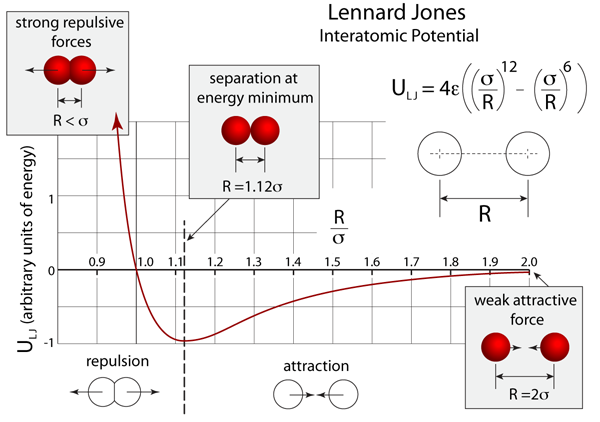
\includegraphics[height=8cm,keepaspectratio, width=\textwidth]{img/LennardJonesFull.png}
\end{center}


En el gráfica se pueden observar dos regiones separadas que representan las fuerzas opuestas de la ecuación. 
Estos segmentos están separados por un valor mínimo que se corresponde con el equilibrio entre el componente repulsivo y el de atracción. 
La distancia de equilibrio (que toma un valor de $2^{1/6}\approx1.12$) se obtiene derivando el potencial e igualándolo a 0.

En el primer segmento de la curva ($r<1.12\sigma$), el valor del potencial esta gobernado por el componente repulsivo. 
Este valor aumenta exponencialmente al disminuir la distancia, toma un valor $V=0$ cuando $r=\sigma$, y se hace positivo para valores de $r<\sigma$ indicando una fuerza repulsiva entre los átomos.

En el punto de equilibrio ($r=1.12\sigma$) el potencial toma el valor mínimo $V=-\epsilon$.

En el segundo segmento de la curva ($r>1.12\sigma$), el valor del potencial esta gobernado por el componente atractivo. El valor del potencial (siempre negativo, indicando una fuerza de atracción) se acerca a 0 a medida que la distancia se acerca a infinito. 


A partir de la forma que toma el potencial de L-J resulta razonable pensar que, si se desprecia el de este potencial para interacciones entre partículas a una distancia mayor que cierto valor de corte, se podrá obtener una buena aproximación del comportamiento a la vez que se reduce considerablemente la cantidad de cálculos necesarios en cada paso de la simulación.
Esta es una aproximación que proveen varias de las versiones implementadas del método, permitiendo que el usuario defina un valor de cutoff. 
En cada paso, si dos partículas están separadas por una distancia mayor que el cutoff se les asigna automáticamente un valor de potencial $V_{LJ}=0$ asumiendo que se está realizando una buena aproximación, lo que elimina el costo de tener que calcular el valor real. 
Depende del usuario definir un cutoff que sea coherente con el sistema y simulación a realizar.

Como se mencionó previamente, el potencial de L-J genera una aproximacion relativamente buena de las interacciones de no union en modelos moleculares y, dada su simplicidad, es incluido en gran parte de los campos de fuerzas utilizados en dinámica molecular.
Es por eso que la optimización del calculo asociado tendría un gran impacto en este métdodo de simulación. Además, la forma funcional implica que existe, al menos débilmente, entre todos los pares de particulas del sistema, lo que se traduce en una gran cantidad de cálculos por paso. 
El cálculo de este potencial representa así la mayor parte del costo computacional asociado a la simulación. 


\subsection{Condiciones de frontera}

Hasta aquí hemos definido al sistema como el conjunto de átomos sobre los cuales realizamos la simulación. 
Sin embargo, los sistemas reales tienen, en términos practicos, un tamaño infinito. 
Es decir, independientemente de cuántos elementos podamos incluir en nuestro conjunto de simulación, el número de parículas(N) será siempre despreciable con respecto al nuúero de componentes del sistema macroscópico real.

Si no se implementa ninguna condición particular a los límites de nuestro sistema, se estaría simulando un conjunto de particulas que se encuentra en el vacío. 
De esta forma, las interacciones ocurrirían solo entre las particulas del conjunto de simulación que definimos, sin tener en cuenta ningún elemento en el contexto.
Además, no habría limites definidos para las posibles posiciones de las partículas, las cuales pueden, por lo tanto, difundir libremente durante la ejecución.

Este tipo de simulaciones raramente es útil ya que no representan situaciones realistas. Se debe tener en cuenta, entonces, condiciones especiales que tendrán los limites en la simulación para que estos representen de forma adecuada a los sistemas de interés.
Existen distintas aproximaciones para implementar estas condiciones en los límites manteniendo un conjunto reducido de particulas. 

Utilizar condiciones periódicas de borde es la forma mas común de simular un sistema infinito. Aplicando esta condición, las partículas están contenidas en una caja de simulación con un tamaño definido. 
Esta caja es replicada virtualmente al infinito en las tres direcciones del eje cartesiano, llenando completamente el espacio.
Todas las imágenes de las partículas se mueven de forma idéntica a la partícula central. De hecho, sólo una de ellas(la que se encuentra en la caja central) es la que efectivamente se está simulando.
Cuando una partícula entra o sale de la caja central, una imagen de ella entra o sale por la cara opuesta de esta región, de manera tal que el número de partículas contenidas en la región de simulación siempre se conserva.
Se puede ver que, de esta forma, los límites del sistema que se está simulando son virtualmente eliminados y no tienen ningún efecto sobre la simulación.
Como resultado de esto, cada partícula perteneciente al conjunto de simulación interactúa no solo con las demás partículas de este, sino también con las imágenes virtuales que estamos teniendo en cuenta.

Al parecer, el número de interacciones (y por lo tanto la cantidad de cálculos a realizar) se incrementará enormemente con esta nueva condición. 
Sin embargo, esto puede evitarse si se utiliza un potencial con un rango finito, dado que en este caso se pueden ignorar las interacciones entre partículas separadas por una distancia mayor a cierto valor de cutoff.
En este caso, teniendo un valor de cutoff $R_{c}$ y definiendo una caja de simulaciún cuyo lado menor tenga una longitud $L_m$: 
Si hacemos cumplir que $L_m>2R_{c}$, entonces se verá que, como máximo, solo una de las imágenes de cada particula quedará dentro del rango del cutoff y por lo tanto debera ser considerada.
Este método, conocido como el criterio de imagen mínima, permite limitar el número de cálculos necesarios considerando solo la imagen mas cercana e ignorando el resto. 
De esta forma se puede cumplir con las características infinitas del sistema real y las propiedades impuestas por el potencial, logrando una mejor aproximación en la simulación.
La figura \ref{minimage} muestra una representación gráfica de este método. 


\begin{figure}[!ht]
\centering
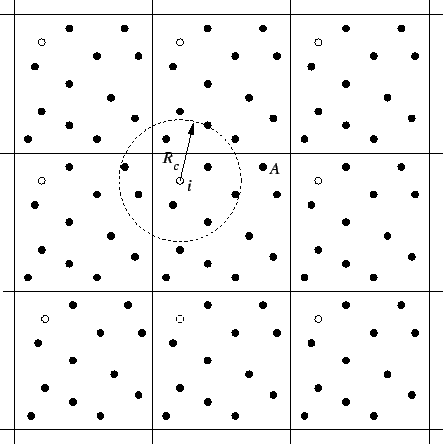
\includegraphics[keepaspectratio, height=10cm ,width=0.5\textwidth]{img/minimage.png}
\caption{Criterio de imagen mínima para condiciones periódicas de frontera. Los círculos sin relleno representan todas las imágenes de la misma particula i}
\label{minimage}
\end{figure}


% propiedades fisicas van a depender del tamano de la caja
% Agregar detalles de sumatoria de Ewald ?










\subsection{Estado del arte}



Desde que fue desarrollado, el método ha sido de una gran utilidad  y ha demostrado una posiblidad de aplicación a futuro mucho mayor. 
Esta posiblidad de aplicarlo a sistemas cada vez mas grandes y procesos en escalas de tiempo mayores es lo que impulsó una constante búsqueda de mejoras sobre el algoritmo inicial.
Se han desarrollado entonces una gran cantidad de estrategias que apuntan a optimizar el costo computacional asociado al método, sin sufrir una pérdida considerable en la precisión.

Para sistemas típicos de biomoleculas en donde el sistema está compuesto por una macromolécula(ej. proteínas) rodeada de un solvente líquido, es posible utilizar una aproximación conocida como solvente implicito.
% referencia : Born solvation model [V. Tsui  D.A. Case, Biopolymers (Nucl. Acid. Sci.) 56, 275-291 (2001)].
En este modelo, el solvente se representa como un medio continuo alrededor del sistema central en lugar de representar explícitamente todas las unidades que lo componen, reduciendo considerablemente el número de cálculos necesarios para evaluar la interacción con las moléculas de solvente. Al ser una aproximación, tiene ciertas limitaciones en cuanto a la precisión y al tipo de sistemas en los que puede ser aplicado.

El calculo asociado al componente electroestatico puede ser optimizado usando el método conocido como sumatoria Ewald. Este metodo permite aproximar el calculo de interacciones que actuan en un amplio rango de distancias sobre sistemas periódicos. 

Otra adaptación muy utilizada es la implementación de una lista de vecinos para cada partícula. Esta lista mantiene las moleculas que estan dentro del rango de interaccion(distancia menor al cutoff) y son los unicos que se tendran en cuenta a la hora de hacer el calculo. La optimización se basa en que la lista solo se actualiza cada una cantidad de pasos definida como parámetro. 
Este valor se deriva experimentalmente a partir de simulaciones de prueba y es el parámetro que balancea la optimización y la precisión: cuanto mas se demora la actualizacion mejor es el tiempo de ejecución pero menos representativa es la lista acerca de la realidad del entorno y, por lo tanto, menos preciso es el calculo.

Existe una gran cantidad de variantes del algoritmo, solo se han mencionado algunos de los caminos en los que se ha avanzado realizando modificaciones con respecto a la descripcion inicial.

En cuanto a las arquitecturas de cómputo, las implementaciones sobre GPU, que son el centro de este trabajo, se han establecido como estándares para las implementaciones del algoritmo. 
Esto se debe al gran poder de cómputo que proveen en relacion al costo económico, teniendo en cuenta que el algoritmo es altamente paralelizable y este tipo de hardware provee las condiciones necesarias para su implementacion.

Con este contexto , las capacidades de cálculo actuales permiten realizar simulaciones de dinámica molecular en sistemas de hasta XXXXXXX átomos aproximadamente, sobre un intervalo de tiempo del orden de YYYYYYY  micro/pico/******segundos).

Si bien se ha avanzado mucho desde el desarrollo del método, existen múltiples procesos de interés que podrían ser abordados mediante experimentos de simulación computacional pero que el intervalo de tiempo en el cual ocurren no es posible de ser alcanzado con los recursos disponibles hoy en dia.
Esta situación hace que se destine una gran cantidad de esfuerzo para continuar las mejoras en el método y mantener las implementaciones a la par de las arquitecturas disponibles.
El presente trabajo intenta, entonces, adecuar las implementaciones más actuales del método para explotar al máximo todas las características que ofrece la arquitectura de GPU. 
















% LO DEJO PARA ESCRIBIR MAS ADELANTE: ACÁ VA LA DESCRIPCION GENERAL DE LA ARQUITECTURA Y ALGUNOS DETALLES QUE USO EN LAS IMPLEMENTACIONES 
\chapter{La arquitectura GPU}











\chapter{Algoritmos}
\begin{comment}
 
PRIMERO HAY UNA PARTE GENERAL DE ´INTRODUCCION´:  EN ESTA PARTE TENGO QUE ACLARAR BIEN LOS FUNDAMENTOS DE LA MODIFICACION 
-EN PRIMER LUGAR TENGO QUE EXPLICAR QUE ES LO QUE YA EXISTE EN CUANTO A IMPLEMENTACIONES DE DINAMICA MOLECULAR (AMBER GPU, ETC). P 
PUEDO ARRANCAR ´ASUMIENDO´ QUE LA IMPLEMENTACION SECUENCIAL ES CASI OBVIA Y DIRECTA A PARTIR DE LA ESPECIFICACION QUE SE DIO EN LA INTRODUCCION.
-DESPUES EXPLICO POR QUE SE PUEDE PENSAR QUE USANDO LA GPU (Y ASUMIENDO LA IMPLEMENTACION SOBRE GPU COMO BASE) PUEDO USAR UNA TABLA PARA BUSCAR LOS RESULTADOS DE LA FUNCION (POTENCIAL L-J). ACA PUEDO DECIR QUE LA TABLA PUEDE SER IMPLEMENTADA EN CUALQUIER SISTEMA DE MEMORIA. ES DEICR, SI BIEN SE PUEDE IMPLEMENTAR SOBRE CPU ESTA SOLUCION (Y DE HECHO LO HICE) USAMOS LA GPU POR LA MEMORIA DE TEXTURA Y POR SER HOY EN DIA UN ESTANDAR EN LO QUE RESPECTA A DINAMICA MOLECULAR

DESPUES DE LA INTRODUCCION ARMO UNA SECCION (3.1, 3.2, etc) PARA CADA UNA DE LAS VARIANTES. AHI DETALLO CADA VARIANTE:
SOLO ARMO 3 SECCIONES: EL ALGORITMO BASE DONDE EXPLICO TODO, EL ALGORITMO QUE USA UNA TABLA CON EL POTENCIAL, Y EL ALGORITMO QUE USA UNA TABLA CON EL VALOR DE LAS DERIVADAS.
DESCRIBO LOS ALGORITMOS IMPLEMENTADOS, AGREGANDO CUALQUIER DETALLE QUE HAGA FALTA (QUE NO ESTE EN LA INTRODUCCION DE DINAMICA MOL.).
LA PARTE DE PERIODICIDAD LA EXPLICO ACA???


****
TENGO UNA LINEA ACA QUE TRAJE DE OTRO LADO, NO SE DONDE METERLA:
Existen diversas implementaciones del algoritmo de dinamica molecular con diferentes modelos de interaccion. Las distintas implementaciones existentes involucran al potencial de Lennard-Jones como aporte para evaluar las interacciones de no-union y, en todos los casos, el calculo de este tipo de interacciones representa la mayor parte del costo computacional asociado al método. Se espera entonces que las modificaciones estudiadas en este trabajo puedan ser integradas en diversas implementaciones existentes obteniendo una mejora considerable en la performance.
*****

\end{comment}


% **********SUPUESTAMENTE EN LA INTRODUCCION YA HABLE DE LOS AVANCES QUE HUBO EN EL METODO EN SI, ES DECIR, TODAS LAS OPTIMIZACIONES QUE HAY BASADAS EN MODIFICAR EL ALGORITMO
% ************  ADEMAS, INTRODUJE LA IDEA QUE LAS IMPLEMENTACIONES DEL ALGORITMO SE HAN MANTENIDO AL DIA CON LAS ARQUITECTURAS Y NUEVOS MODELOS DE COMPUTO EXISTENTES
% ****		ACA TENDRIA QUE HABLAR DE LA EVOLUCION (ESTADO DEL ARTE?) DE LAS IMPLEMENTACIONES EN SI, TENIENDO EN CUENTA LA EVOLUCION DE LA ARQUITECTURA, HASTA DEJAR EN CLARO
% 		QUE LA IMPLEMENTACION SOBRE GPU ES EL STANDAR HOY EN DIA*** 




% ***ESTE PRIMER PARRAFO QUE DICE QUE LAS IMPLEMENTACIONES SOBRE GPU SON UN ESTANDAR ....*****LO SAQUE DE LA PARTE DE OBJETIVOS**
.......en primer lugar se hace un algoritmo con caracteristicas similares al estandar del metodo de hoy en dia, pero en su lugar solo implementa un modelo de interaccion de L-J. 
Esto se hace con el objetivo de aislarse de otras implementaciones, de tener una aplicacion general, etc,......


A partir de la descripción del método presentada en el capitulo 1 se puede llegar a una implementacion secuencial en forma casi directa. Este tipo de versiones son las que se utilizaron inicialmente para realizar las simulaciones.
La utilidad que ha mostrado esta técnica desde sus inicios y la posibilidad que ofrece para nuevas aplicaciones hizo que se desarrollen diversas implementaciones para aprovechar los nuevos modelos de computo disponibles, los cuales han avanzado considerablemente teniendo en cuenta que la tecnica fue creada hace ya un largo tiempo. 
Entre los nuevos algoritmos, una gran cantidad se ha enfocado en explotar las caracteristicas intrinsecamente paralelas del metodo. En los ultimos años, con avance de las arquitecturas de GPU y su utilizacion para computo de proposito general, estos algoritmos han sido portados para adaptarse a las caracteristicas propias de GPGPU.
De las versiones mencionadas en el capitulo 1, gran parte de ellas han sido portadas para poder ejecutarse sobre estas arquitecturas. (referencias amberGPU?? gromacs gpu??).

En el capitulo anterior se mostraron las ventajas que brinda el metodo de GPGPU para aplicaciones altamente paralelizables. De la misma forma,  la implementacion del metodo de dinamica molecular sobre esta arquitectura resulta en un aumento muy importante en la performance en forma casi directa. Además de las mejoras en la performance, el bajo costo del hardware en relacion a su poder de computo que provee la arquitectura hace que estas implementaciones sean un estandar de uso en el area.  

De esta forma, hoy en dia se puede encontrar una gran variedad de software para simulaciones de dinamica molecular implementado sobre GPU. A pesar de la gran cantidad de modificaciones que se han agregado y la evolucion en el hardware existente, se sigue dedicando un gran esfuerzo para continuar optimizando el algoritmo con el fin de poder simular nuevos procesos y sistemas de interes que requieren una mayor cantidad de calculos. 
Si se analizan las implementaciones que se utilizan actualmente, se puede ver que la mayor parte del costo computacional del metodo se mantiene asociado al calculo de las interacciones de no-union(entre particulas que no forman enlaces quimicos entre si), el cual esta representado principalmente por el potencial de L-J. Este calculo tiene una complejidad de orden N2 sobre el numero de particulas del sistema....
En el capitulo 1 se describio una aproximacion muy utilizada para intentar reducir la cantidad de calculos necesarios, la cual consiste en despreciar las interacciones entre particulas que se encuentren a mayor distancia que cierto valor de cutoff. Esta aproximacion esta basada en las propiedades de la funcion que describe el potencial de L-J. Incluso ajustando el valor de cutoff a valores suficientemente chicos, el costo que implica este paso representa la mayor parte de los requerimiento......Por esta razon, una gran parte de los esfuerzos se centran en optimizar esta etapa.
 

% ****HASTA ACA YA DEFINI QUE LAS IMPLEMENTACIONES SOBRE GPU SON EL ESTANDAR HOY EN DIA, Y QUE SE HA OPTIMIZADO POCO DEL CALCULO DEL POTENCIAL DE LENNARD-JONES PERO SI DE OTROS ASPECTOS, INCLUSO SE HA OPTIMIZADO EL CALCULO DE LAS INTERACCIONES ELECTROSTATICAS***

% ****AHORA EXPLICO CUALES SON LAS CARACTERISTICAS DE LA FUNCION DE L-J QUE HACEN QUE PUEDA SER TABULADO Y DAR UNA BUENA APROXIMACION 
% DESPUES EXPLICO QUE LAS CARACTERISTICAS DE LA MEMORIA DE TEXTURA ENCAJAN JUSTO PARA IMPLEMENTAR LA TABLA Y LA BUSQUEDA EFICIENTE DEL RESULTADO ASOCIADO***


Como se puede apreciar a partir de la descripcion de este potencial en el capitulo 1, la forma funcional que lo describe se caracteriza por tener un rango de distancias donde el resultado crece(o decrece) exponencialmente, y un punto a partir del cual converge y el valor asociado a la interaccion se hace despreciable.
Basandose en estas caracteristicas es razonable pensar que, utilizando una tabla conteniendo los resultados para un rango de valores definido y, aun sin tener ésta un tamaño excesivo, se podria obtener una buena aproximacion del resultado para cualquier distancia. 


% ****ACA PONGO LAS CARACTERISTICAS QUE OFRECE LA GPU Y QUE PUEDEN SER USADAS APROVECHANDO QUE HOY EN DIA LA MAYORIA DEL SOFT. ESTA IMPLEMENTADO SOBRE GPU*****

Para implementar este mecanismo hay varias propiedades del sistema de memoria que se puede usar y que se deben analizar......................................................



% ****ALGO MAS ANTES DE TERMINAR***

Se debe tener en cuenta que, aún cuando sea posible realizar una buena aproximacion utilizando tablas, el algoritmo de dinamica molecular implica utilizar este valor para obtener las fuerzas y movimientos resultantes de la interaccion, lo cual afecta la posicion (y por lo tanto el valor del potencial asociado) en la proxima iteracion. De esta forma, los errores resultantes de la aproximacion por utilizar tablas de valores seran propagados a lo largo de una simulacion que involucra miles de pasos.....


% ****TERMINO CON****

Asi, en este trabajo se estudiarán distintas formas de utilizar el sistema de memoria de la gpu para realizar el calculo del potencial de Lennard Jones, analizando su utilizacion en el contexto del método de dinamica molecular. Dado que el calculo de este potencial representa la mayor parte del costo asociado a la simulacion, se espera obtener una mejora considerable en el tiempo de ejecución con respecto al algoritmo estandar sobre GPU, el cual resuelve la ecuacion de L-J para cada interaccion a evaluar.


% ESTO DONDE LO PONGO?? LO TRAJE DE LA INTRODUCCION
Es importante destacar que las adaptaciones que se plantean y analizan en este trabajo constituyen una modificación puntual para realizar el calculo del potencial de Lennard-Jones y, por lo tanto, tienen la capacidad de ser incluidas directamente en cualquier algoritmo existente y combinadas junto con cualquier otro método de optimización.
Además, como se vio en el capitulo 1, existen pocas variantes para optimizar el calculo de este potencial de no-union que, además, tiene la característica de ser una de las etapas mas costosas del método en terminos computacionales.

\begin{comment}

**********************************
EN ESTAS SECCIONES DEBERIA HACER UNA DESCRIPCION GENERAL DE LOS 3 ESQUEMAS QUE DESARROLLO(DESPUES CADA UNO PUEDE LLEVAR A 1 O MAS IMPLEMENTACIONES Y VARIANTES).  
-EN EL ALGORITMO QUE USA LA TABLA DEL POTENCIAL SIMPLEMENTE PONGO QUE USO UNA TABLA DONDE POR CADA VALOR DE DISTANCIA TENGO ASOCIADO UN VALOR, QUE A PARTIR DE AHI TENGO QUE AGARRAR 2 VALORES DE LA TABLA PARA PODER OBTENER LA DERIVADA, PUEDO AGREGAR QUE LA VENTAJA DE TENER TABULADO EL VALOR DEL POTENCIAL ES QUE SI QUIERO CALCULAR EL POTENCIAL TOTAL SOLO TENGO QUE LEER 1 DATO DE LA TABLA....BLA BLA.....NO MUCHO MAS.
-EN LA OTRA VERSION, DONDE TENGO TABULADA LA DERIVADA, TENGO QUE EXPLICAR PRIMERO POR QUE NECESITO LA DERIVADA (SUPUESTAMENTE ESTO YA TIENE QUE ESTAR BASTANTE CLARO), 
\end{comment}







\section{Algoritmo base sobre GPU (o Esquema general del algoritmo)}


% ***PUEDO ARRANCAR DE UNA EXPLICANDO EL ALGORITMO Y DESPUES COMENTO LA VENTAJA DE TENER ESTA IMPLEMENTACION ****


El algoritmo inicial sigue la especificacion que se detallo en el capitulo 1....
Dado que el aporte al campo de fuerzas que nos interesa es el correspondiente al potencial de L-J (potencial de no union), este es el unico aporte que se va a considerar. De esta forma, el sistema evoluciona en el tiempo a partir de las velocidades iniciales de las particulas y las fuerzas que se derivan de este potencial, unicamente. Si bien este modelo (considerando solo la interaccion de L-J) no es de utilidad para simular sistemas biologicos de interes (donde existen diversos enlaces entre los elementos), en este caso 


% Esta linea no se si va aca o la pongo directamente en la parte de implementacion
El esquema general del algoritmo se mantiene en todas las variantes. Las modificaciones estan centradas en la etapa de calculo del potencial, el contexto de este se mantiene siempre igual.


Si bien el codigo aqui implementado ya está implementado como parte de distintos paquetes de software de dinamica molecular, el objetivo de realizar un algoritmo independiente, donde la evolucion temporal ocurra unicamente en base al potencial de L-J 

Dado que el trabajo se centra puntualmente en modificar la forma en que se calcula el potencial de L-J, el primer paso consiste en implementar un algoritmo de dinamica molecular que utilice exclusivamente este modelo de interaccion. 
Es decir, el campo de fuerzas estará definido exclusivamente por el potencial de Lennard-Jones que modela interacciones de no-unión. 
De esta forma, no será posible simular (de forma correcta) sistemas moleculares que incluyan enlaces químicos, ya que estos no estarán correctamente modelados por el campo de fuerzas. 

El objetivo de esto es, en primer lugar, facilitar la implementacion de esta modificacion/optimizacion en el algoritmo, y en segundo lugar probar las propiedades de esta variante de forma independiente a cualquier otra implementacion existente sobre GPU. 
Utilizando una implementacion propia se puede evaluar, de forma aislada, las ventajas y desventajas del uso de una tabla numerica. De esta forma se puede verificar facilmente que las variaciones en el tiempo y en la precision de los resultados son producto exclusivo de las modificaciones implementadas en cada paso.

Idealmente, las ventajas resultantes de este trabajo se sumaran a las caracteristicas de cualquier implementacion existente. 


% ****describo brevemente el algoritmo*****


% *****ACA METO LO DE PERIODICIDAD???***
% **PUEDO EXPLICAR EN FORMA ABSTRACTA CUAL ES LA IDEA DE LA PERIODICIDAD, MASOMENOS QUE TENGO QUE TENER EN CUENTA A LA HORA DE IMPLEMENTARLO EN EL ALGORITMO, EL RESTO LO EXPLICO EN LA PARTE DE IMPLEMENTACION*** 





\section{Calculo usando tablas de valores del potencial }


% Tengo que explicar que el potencial de Lennard Jones depende del par de elementos que interaccionan (y por lo tanto va a haber tablas de LxL )



\section{Calculo usando tablas de valores de la derivada  }


















\chapter{Implementaciones}
\begin{comment}
Aca describo el kernel y aspectos relevantes de las versiones implementadas:
-que variables tengo que tener en cuenta en las implementaciones(por ej. el tamaño de la tabla,el rango, etc)
-que resultados espero!!!!
-como afecta la periodicidad. la describo aca o en el capitulo anterior??
-como afecta el tamaño de los bloques
\end{comment}

\section{Esquema general de la implementación}
\section{Implementacion sobre CPU}
\section{Implementación usando tabla de valores potenciales}
% \subsubsection{Tabla sobre memoria global}
% \subsubsection{Tabla sobre memoria de textura}
\section{Implementación usando tabla de derivadas}
% \subsubsection{Tabla sobre memoria global}
% \subsubsection{Tabla sobre memoria de textura}













\chapter{Resultados}
\section{Sistemas de partículas utilizados}
\section{Performance}
\subsection{Evaluación de las implementaciones}
\subsection{Efectos del tamaño de bloque}
\section{Calidad numérica}














\chapter{Conclusiones}















\end{document}
